\chapter{Proiectare rețele profile de profile subtiri}\label{chapter:proiectare}

\section{Alegerea razei retelelor}

Pentru proiectarea retelelor de profile se calculeaza intai raza medie a retelelor la care se vor face in continuare calculele triunghiurilor de viteze. Se alege pentru aceasta o raza medie $R_m$ intre raza de periferie si raza de butuc astfel incat debitul dintre cele doua zone sa fie egale:

\begin{equation}
\frac{Q}{2} = V_a \pi (R_p^2 - R_m^2) \Rightarrow{} R_m = \sqrt{\frac{R_p^2 + R_b^2}{2}} = 
\end{equation}


Considerăm zona de interacțiune a turbinei cu fluidul în trei porțiuni:
\begin{itemize}
	\item prima zonă numită zonă amonte stator ZAS
	\item a doua porțiune: zona stator-rotor numită de acum ZSR
	\item zona trei sau zona aval rotor ZAR
\end{itemize}

La ZAS avem viteza axială $V_{a}$ care se menține pe toate cele trei porțiuni considerate ale turbinei, iar valoarea acesteia este:

\begin{equation}
V_a=\frac{Q}{\pi(R_{p}^2-R_{b}^2)}=6.8\si{m/s}
\end{equation}

\În ZSR, avem viteza tangențiala $U$:

\begin{equation}
U=\omega R_m \text{ sau } \frac{\pi n}{30} R_m=16.0\si{m/s}
\end{equation}

Conform ecuației fundamentale a turbomașinilor (ecuația lui Euler) avem viteza absolută:

\begin{equation}
gH=UV_{u}, \text{ sau } gH=\frac{\pi n}{30} R_m V_{u} \Rightarrow V_{u} = \frac{30gH}{\pi n R_m} = 14.7\si{m/s}
\end{equation}


Unghiul $\alpha_2$ dintre direcția tangențială și viteza absolută $V_u$ este:

\begin{equation}
tan(\alpha_{2 })=\frac{V_{a}}{V_{u}} \Rightarrow \alpha_{2}=65.1\si{\degree}
\end{equation}



Unghiul $\beta_2$ dintre direcția tangențială și viteza relativă $W_2$ este:

\begin{equation}
tan(\beta_{2})=\frac{U - V_u}{V_a} \Rightarrow \beta_{2} =11.0\si{\degree}
\end{equation}


\section{Triunghiurile de viteză}

Triunghiurile de viteză pentru ZSR arată în felul următor:

\begin{figure}[h!]
	\centering
	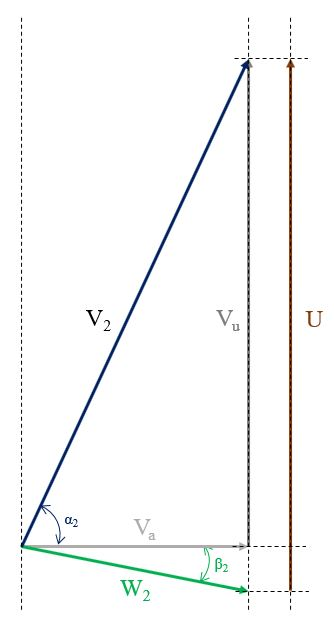
\includegraphics[scale=0.5]{figures/triunghi_viteza_ZSR.jpg}
	\caption{Triunghi viteză în zona stator-rotor}
	\label{Triunghi viteză în zona stator-rotor}
\end{figure}



Pentru ZAR avem aceleași viteză axială $V_a$ respectiv tangențială $U$. Putem calcula unghiul $\beta_3$ pentru a completa triunghiurile de viteză.

\begin{equation}
tan(\beta_{3})=\frac{U}{V_a} \Rightarrow \beta_{3} =66.9\si{\degree}
\end{equation}

\begin{figure}[t!]
	\centering
	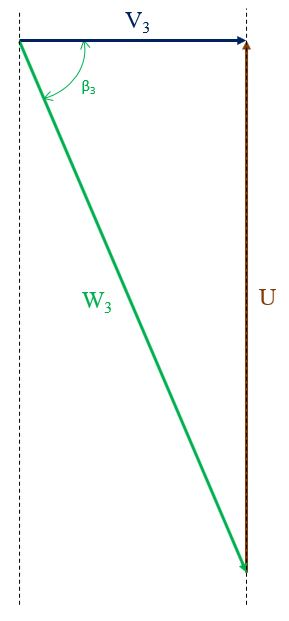
\includegraphics[scale=0.5]{figures/triunghi_viteza_ZAR.jpg}
	\caption{Triunghi viteză în zona aval rotor}
	\label{Triunghi viteză în zona aval rotor}
\end{figure}

\clearpage


\section{Adăugare funcție de grosime}

\subsection{Subsection}